\chapter{Wprowadzenie}
\section{Tytyna}
Tytyna lub też inaczej konektyna jest największym poznanym do tej pory białkiem, które składa się z około 30000 aminokwasów. Stanowi ono jeden ze składników sarkomerów i odgrywa ważną rolę w ich pracy~\cite{parametry, Maruyama_1997}.

Sarkomer stanowi podstawowy element budulcowy mięśni poprzecznie prążkowanych i odpowiedzialny jest za ich kurczliwość. Na podstawie obrazu z mikroskopu optycznego podzielony został na pasma I (od izotropowe) oraz pasma A (od anizotropowe). Zbudowany jest z leżących naprzeciwko siebie filamentów aktyny oraz miozyny, które są przyłączone do dysku Z oraz linii M. Aktyna oraz miozyna odpowiadają za skurcze sarkomerów. Pojedyncza cząsteczka tytyny rozciąga się na długości około 1 $\mu$m od dysku Z do linii M sarkomeru.\cite{Labeit_1995} 

\begin{figure}[h!]
\begin{centering}
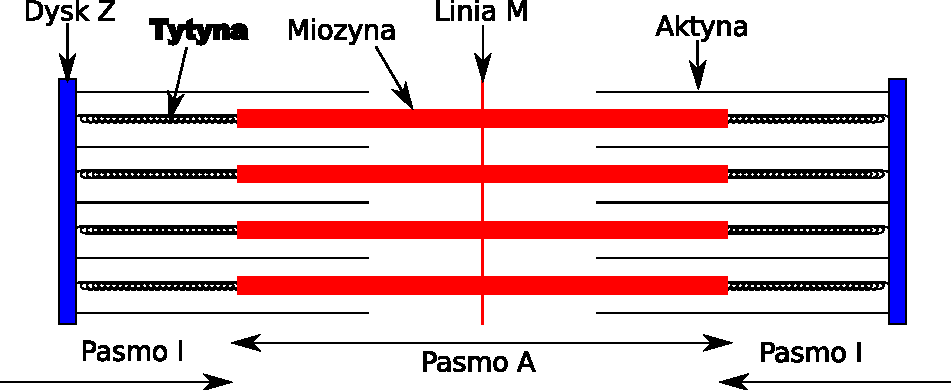
\includegraphics[width=300px]{./rys/sarko.pdf}
\caption{Schemat budowy sarkomeru.}
\end{centering}
\end{figure}

Tytyna składa się z około 300 powtórzeń domen fibrynokonektyny \mbox{typu~III~(Fn-3)}, która znajduje się tylko w paśmie A oraz domen immunoglobuliny (Ig), które występują wzdłuż całej jej długości. W skład wchodzi także obszar PEVK w pasmie I, który nie posiada jednej, stabilnej struktury. Długość regionu PEVK oraz ilość domen Ig w paśmie I waha się znacznie w zależności od miejsca występowania mięśnia poprzecznie prążkowanego w organizmie. Dla przykładu w mięśniach szkieletowych stwierdzono występowanie 90 domen Ig przy regionie PEVK składającym się z 2174 aminokwasów, kiedy w mięśniu sercowym wartości te wynoszą 37 domen Ig oraz 163 aminokwasów regionu PEVK\cite{Labeit_1995}.

\begin{figure}[h!]
\begin{centering}
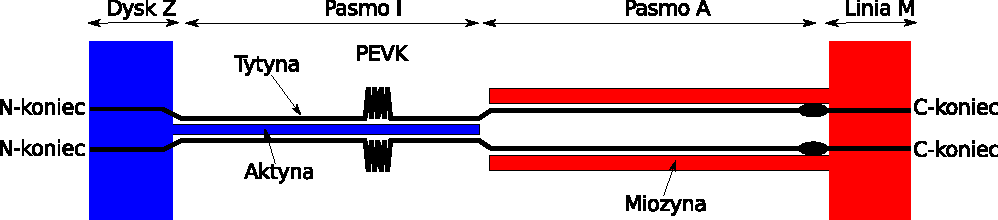
\includegraphics[width=400px]{./rys/tytyna.pdf}
\caption{Model tytyny w sakromerze.}
\end{centering}
\end{figure}

Podczas skurczu mięśnia tytyna odpowiada za utrzymanie elementów budulcowych sarkomeru. Podczas rozciągania natomiast gromadzi w sobie powstające naprężenia, przeciwdziała zerwaniu oraz powoduje powrót do stanu wyjściowego po ustaniu zewnętrznej siły powodującej rozciągnięcie. Stwierdzono, że obszar PEVK odpowiada za elastyczność tytyny przy niskich rozciągnięciach. Po rozwinięciu tego obszaru stabilnie pofałdowane domeny Ig stawiają opór dalszemu rozciąganiu powodując wzrost naprężenia. Tego typu mechanizm podwójnej sprężyny wyjaśnia niejednorodny wzrost naprężenia przy rozciąganiu pojedynczego sarkomeru.

W tej pracy szczególna uwaga poświęcona została kinazie tytyny, której struktura została dokładnie zbadana\cite{Tit_stru} oraz istnieje szereg publikacji z danymi eksperymentów AFM oraz symulacji dynamiki molekularnej\cite{mechanoenz, 1tki}. Białko to znajduje się blisko C-końca tytyny, w linii M. Polipeptyd ten składa się z 321 aminokwasów. Podczas powstawania naprężenia w mięśniu część tego naprężenia przekazywana jest na kinazę tytyny prowadząc do częściowego jej rozwinięcia, które powoduje odsłonięcie jej centrum aktywnego. Aktywna kinaza katalizuje fosforylację innego białka mięśniowego, telethoniny, które odgrywa rolę przy tworzeniu się mięśni, a także wpływa na ekspresję genów\cite{Kin_geny}. W ten sposób kinaza ta spełnia rolę molekularnego czujnika naprężenia.

\begin{figure}[h!]
\begin{centering}
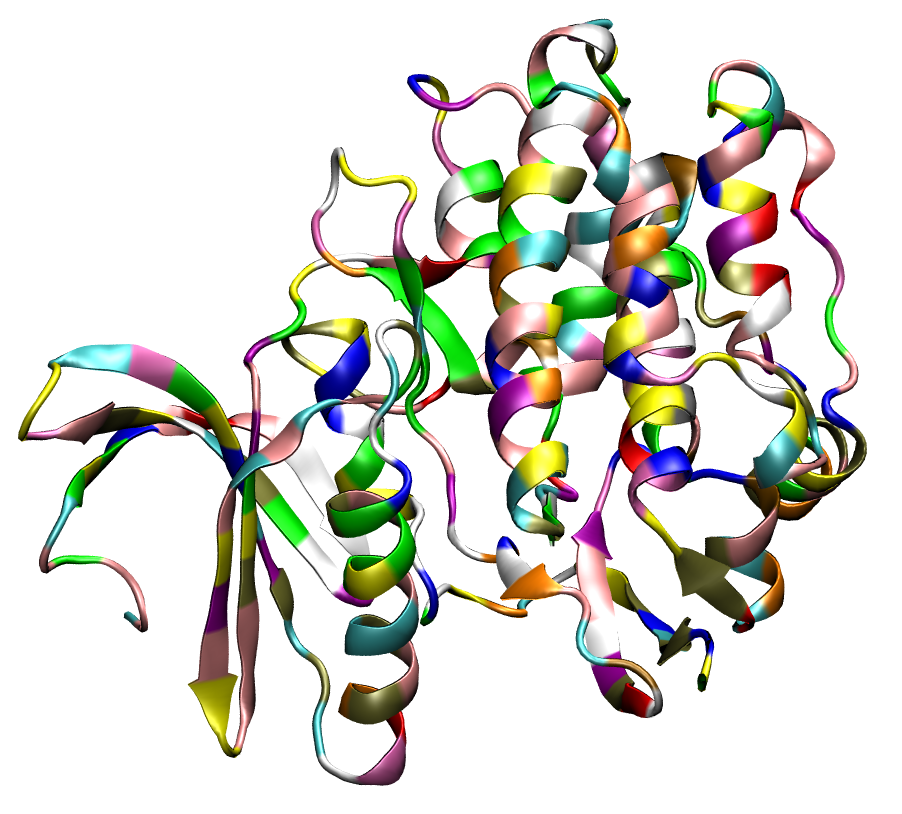
\includegraphics[width=300px]{./rys/plot_tki.png}
\caption{Wizualizacja struktury trzeciorzędowej domeny kinazy tytyny.}
\end{centering}
\end{figure}

\section{AFM}

Jednym z narzędzi, które pozwala na uzyskanie danych dla pojedynczych cząsteczek jest mikroskop sił atomowych (ang. Atomic Force Microscope --- AFM). W omawianych w tej pracy eksperymentach mamy do czynienia z cząsteczkami przytwierdzonymi do ostrza mikrodźwigni (ang. cantilever) z jednej strony, a do podstawy z drugiej. Następuje ruch podstawy w pionie i mierzone jest odchylenie sprężystego ramienia za pomocą wiązki laserowej. Na tej podstawie obliczana jest siła działająca na badaną cząsteczkę. W zależności od rodzaju eksperymentu możemy mieć do czynienia z rozciąganiem przy stałej sile, dzięki czemu można badać kinetykę reakcji w zależności od przyłożonego naprężenia\cite{Fernandez} albo przy stałej szybkości rozciągania, gdzie można badać miedzy innymi siły zerwania bądź też rozplatania\cite{Carrion-Vazquez30031999, Fisher1999379}. 

\begin{figure}[h]
\begin{centering}
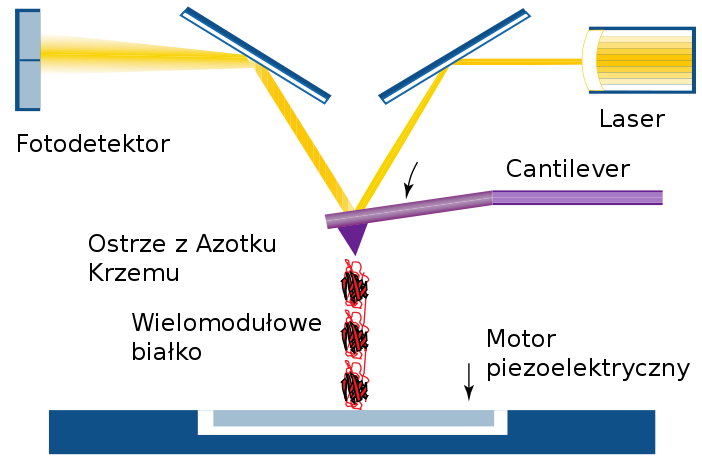
\includegraphics[width=300px]{./rys/afm1.png}
\caption{Schemat eksperymentu AFM.}
\end{centering}
\end{figure}

\section{Symulacje dynamiki molekularnej}

Symulacje dynamiki molekularnej (\textbf{MD} -- ang. Molecular Dynamics) stanowią jeden z działów chemii obliczeniowej (ang. Computational chemistry). W przeciwieństwie do symulacji Monte Carlo symulacje \textbf{MD} mogą być używane także do obliczeń układów nie będących w stanie równowagi oraz do wydarzeń dynamicznych, zachodzących w czasie. Z tego powodu symulacje \textbf{MD} są bardziej uniwersalne i znajdują zastosowanie w omawianym w tej pracy problemie\cite{Gromacs_manual}.

Podstawowym zadaniem, które stoi przed tymi obliczeniami jest rozwiązanie równań ruchu Newtona (\ref{eq:Newton}) dla układu składającego się z $N$ atomów oddziałujących na siebie zarówno za pomocą wiązań chemicznych jak i też za pomocą oddziaływań elektrostatycznych i van der Waalsa.

\begin{equation}m_{i}\frac{\partial ^{2}\vec{r_{i}}}{\partial t^{2}} = \vec{F_{i}}, \hspace*{0.5cm} \text{i}= 1 \ldots N \label{eq:Newton}\end{equation}

Gdzie $m_{i}$ oznacza masę, $\vec{r_{i}}$ wektor położenia, a $\vec{F_{i}}$ siłę działającą na \textit{i}-ty atom.

Dane na temat siły działającej na \textit{i}-ty atom znajduje się obliczając ujemny gradient z funkcji potencjału $V(\vec{r_{1}}, \vec{r_{2}}, \ldots, \vec{r_{N}})$

\begin{equation} \vec{F_{i}} = - \frac{\partial V(\vec{r_{i}})}{\partial \vec{r_{i}}} \end{equation}

Równania te rozwiązywane są numerycznie z małym krokiem czasowym. Co pewien czas w zależności od parametrów symulacji system jest kontrolowany pod względem temperatury oraz ciśnienia. Położenia oraz prędkości atomów są zapisywane w postaci trajektorii. Po początkowych dużych zmianach system po pewnym czasie osiąga stan równowagi. 

Symulacje te posiadają jednak pewne ograniczenia, z których należy zdawać sobie sprawę przy przeprowadzaniu i planowaniu obliczeń.
\begin{description}
\item[Symulacje odbywają się według mechaniki klasycznej] \hfill \\
Rozwiązując równania ruchu Newtona (\ref{eq:Newton}) pomijamy efekty kwantowe. Co za tym idzie symulacje \textbf{MD} nie nadają się do badania mechanizmów reakcji czy też stanów przejściowych. Istnieje jednak możliwość połączenia z programami do obliczeń kwantowomechanicznych, na przykład \textsc{Gaussian}, jednak obliczenia te są bardzo czasochłonne.
\item[Elektrony znajdują się w stanie podstawowym] \hfill \\
Wykorzystywane pola siłowe zawierają definicje oddziaływań atomów w stanie podstawowym. W obliczeniach nie uwzględnia się ruchu elektronów. Z tego powodu wszelkie procesy związane z transferem elektronów oraz te, gdzie stan wzbudzony odgrywa kluczową rolę w eksperymencie nie mogą być w pełni badane.
\item[Pola siłowe są tylko przybliżone] \hfill \\
Pola siłowe zawierają opis oddziaływań pomiędzy atomami w różnych cząsteczkach. Nie uwzględniają jednak możliwości polaryzacji wiązań. 
\item[Oddziaływania są w pewnej odległości ucinane] \hfill \\
Aby uprościć obliczenia oraz aby zapobiec nakładaniu się tych samych oddziaływań przez periodyczność stosuje się ograniczenie ich przy pewnej zdefiniowanej przez parametry symulacji odległości.
\item[Periodyczność pudła] \hfill \\
Aby zapobiec rozpraszaniu się atomów do próżni oraz aby uniknąć nienaturalnie małego układu badawczego wprowadzono periodyczność. Przez periodyczność w tym przypadku należy rozumieć fakt, że jeśli atom wybiega poza granice układu, to automatycznie pojawia się on po przeciwnej stronie. W ten sposób przenoszone są także oddziaływania pomiędzy atomami. Częściowo zbliża to badany układ do kryształu, co może powodować błędy w obliczeniach.
\end{description}
 

\subsection{Gromacs}\

Gromacs stanowi jeden z wielu dostępnych programów do symulacji dynamiki molekularnej, jednak ze względu na ilość materiałów szkoleniowych\cite{Gromacs_tut} i ilość publikacji, w których występuje, właśnie to narzędzie zostało użyte do obliczeń.

Gromacs stanowi pakiet programów do przygotowania symulacji, ich przeprowadzenia oraz analizy wyników. Dostępny jest bezpłatnie, na licencji GNU General Public License. Napisany został przez grupę Hermana Berendsensena (Department of Biophysical Chemistry of Groningen University). Obecnie rozwijany jest przez Erika Lindahla  (Stockholm Center for Biomembrane Research, SE), Davida van der Spoela (Biomedical Centre, Uppsala, SE) oraz Berka Hessa (Stockholm Center for Biomembrane Research, Stockholm, SE). 

Program został domyślnie napisany na systemy Uniksowe, jednak dostępny jest również pod system Windows. Spośród innych narzędzi wyróżnia się przede wszystkim wydajnością wynikającą ze zoptymalizowanego kodu, który wykorzystuje także multimedialne instrukcje procesorów jak MMX czy SSE (ang. Streaming SIMD Extensions) i SSE2. Przy wykorzystaniu bibliotek MPI (ang. Message Passing Interface) możliwe jest wykonywanie obliczeń na kilku jednostkach jednocześnie, co zdecydowanie skraca czas obliczeń. 

\subsection{NAMD}
W wielu publikacjach do symulacji używany jest program NAMD~\cite{NAMD}. Na stronie autorów \cite{namdtut} dostępne są tutoriale, które pozwalają na łatwiejsze wdrożenie się do pracy z tym programem. Jednak dla obliczeń prowadzonych przy zbliżonych warunkach NAMD okazuje się kilkukrotnie wolniejszy od programu \textsc{Gromacs}\cite{NAMD_sux}. Gromacs pozwala na zastosowanie dwukrotnie większego kroku czasowego przy tym samym błędzie obliczeń. Ponadto NAMD wykazuje gorszą skalowalność w porównaniu do Gromacsa i co za tym idzie obserwuje się większy spadek wydajności obliczeń na jednostkę obliczeniową przy wzroście liczby procesorów. Stąd też wybór programu Gromacs jako lepszego narzędzia do prowadzenia symulacji.

\section{Model teoretyczny Hummera-Szabo}

\begin{figure}[h]
\begin{centering}
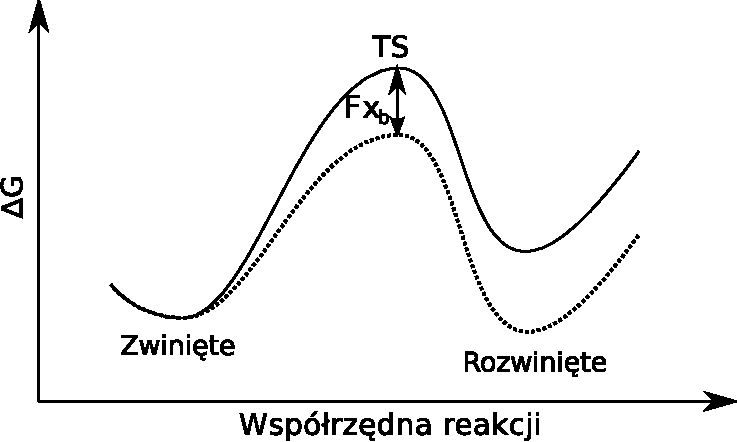
\includegraphics[width=100mm]{./rys/enswob.pdf}
\caption{Schemat ideowy zmiany powierzchni entalpii swobodnej pod wpływem rozciągania.}
\end{centering}
\end{figure}

Podczas rozciągania cząsteczki pod wpływem siły dochodzi do obniżenia bariery energetycznej stanu przejściowego, który cząsteczka musi przekroczyć by ulec rozwinięciu, które następuje w wyniku fluktuacji termicznych. Wprowadzenie siły do układu zwiększa prawdopodobieństwo przekroczenia bariery energetycznej. Do opisu fenomenologicznego tego zjawiska służy równanie Bell'a \ref{eq:bell}.

\begin{equation} k(t)=k_{0} \exp\left( \frac{ F(t)x_{b}}{k_{B}T}\right) \label{eq:bell}\end{equation}

Gdzie $k(t)$ oznacza stałą szybkości rozplatania przy sile $F(t)$, $k_{0}$ stanowi stałą szybkości rozplatania bez obecności siły, $x_{b}$ stanowi odległość bariery od minimum na powierzchni energii swobodnej, $k_{B}$ stanowi stałą Boltzmanna, a $T$ temperaturę bezwzględną.

Model fenomenologiczny zaprezentowany w pracy Hummera i Szabo \cite{Hummer_Szabo_2003} jest jednak niewystarczający do analizy wyników dla szerokiego zakresu szybkości rozciągania, ponieważ istniejące przybliżone rozwiązania analityczne mają zastosowanie tylko do wąskich, eksperymentalnych zakresów szybkości rozciągania i nie mogą być używane do analizy danych dla szybkości używanych w symulacjach.

W przypadku modelu mikroskopowego nie istnieją ścisłe rozwiązania analityczne, jednak przedstawione rozwiązanie numeryczne znajduje zastosowanie dla szerokiego zakresu prędkości. 

W modelu mikroskopowym zakładamy, że siła jest zdefiniowana potencjałem harmonicznym:

\begin{equation} V_{s}(x-vt)=\frac{1}{2} k_{B} T \kappa_{s}\left(x-vt\right)^2 \label{eq:harm}\end{equation}

Gdzie $V_{s}$ oznacza potencjał po współrzędnej reakcji $x$ (odległość ramienia od położenia 0), $v$ prędkość rozciągania, $t$ czas, a $\kappa_{s}$ oznacza stałą siłową wirtualnego cantilevera.

Kształt powierzchni entalpii swobodnej opisany jest zależnością:


\begin{equation} V_{0}(x)=\left\{
\begin{array}{l l} 
\frac{1}{2} k_{B} T \kappa_{m}x^2 & \quad \text{dla } x <  x_{b}\\
- \infty & \quad  \text{dla } x \geqslant x_{b}\\
\end{array} \right.
\label{eq:ent}\end{equation}

Gdzie $\kappa_{m}$ oznacza stałą sprężystości cząsteczki, a $x_{b}$ barierę, po której potencjał spada do $-\infty$.

System porusza się po następującej powierzchni potencjału: 

\begin{equation} V(x,t)=\left\{
\begin{array}{l l} 
\frac{1}{2} k_{B} T \kappa_{m}x^2 +\frac{1}{2} k_{B} T \kappa_{s}\left(x-vt\right)^2& \quad \text{dla } x <  x_{b}\\
- \infty & \quad  \text{dla } x \geqslant x_{b}\\
\end{array} \right.
\label{eq:potencjal_sum}\end{equation}

Zakładamy również, że system porusza się ruchem Browna po powierzchni potencjału wyznaczonej przez \ref{eq:potencjal_sum}. Wobec tego spełnione jest równanie dynamiki Browna:

\begin{equation} \dot{x}=-D \bigtriangledown V (x,t) +R(t)\label{eq:brown}\end{equation}

Gdzie $R(t)$ stanowi losową siłę z rozkładu Gaussa, gdzie jej wartość średnia wynosi 0, a wariancja $\overline{(t)R(t')}=2D\delta(t-t')$.

Po podstawieniu \ref{eq:potencjal_sum} do \ref{eq:brown} otrzymujemy równanie ruchu:

\begin{equation} \dot{x}=-D\kappa_{m} x - D\kappa_{s} (x-vt) +R(t)\label{eq:ruchu}\end{equation}

Przy założeniu, że $\overline{R(t)}=0$ można obliczyć $\overline{x}(t)$, oznaczające średnie położenie w chwili $t$, rozwiązując równianie \ref{eq:ruchu}, które przy pominięciu składnika $R(t)$ przy uśrednianiu przekształca się w równanie różniczkowe pierwszego rzędu. Równianie to rozwiązano przy użyciu programu Wolfram Alpha\cite{wolfram}. Jako rozwiązanie ogólne otrzymano:

\begin{equation} \overline{x}(t)= c_{1}e^{-(\kappa_{m}+\kappa_{s})Dt} + \frac{\kappa_{s}v((\kappa_{m}+\kappa_{s})Dt -1 )}{D(\kappa_{m}+\kappa_{s})^2} \label{eq:rozw_og}\end{equation}

Z warunku $\overline{x}(0)=0$ otrzymujemy współczynnik $c_1$ oraz rozwiązanie szczególne:

\begin{equation} \overline{x}(t)= \frac{\kappa_{s}v((\kappa_{m}+\kappa_{s})Dt + e^{-(\kappa_{m}+\kappa_{s})Dt}-1 )}{D(\kappa_{m}+\kappa_{s})^2} \label{eq:rozw_szczeg}\end{equation}

Aby znaleźć średnią siłę w danym czasie $\overline{F}(t)$ należy posłużyć się równaniem \ref{eq:harm} na zależność potencjału od czasu i położenia. W wyniku obliczenia ujemnej pochodnej po $x$ otrzymujemy siłę.

\begin{equation} \overline{F}(t) = - k_{B}t\kappa_{s} ( \overline{x}(t) -v t)  \label{eq:sila_czas}\end{equation}

Aby znaleźć średnią siłę zerwania należy przyjąć, że zerwanie następuje przy przejściu przez barierę $x_b$, które to następuje po czasie $\tau$. Czas ten można obliczyć z równania \ref{eq:rozw_szczeg} oraz warunku, że średnie położenie w momencie zerwania $\tau$ wynosi $x_b$, czyli $\overline{x}(\tau)=x_b$.

Aby znaleźć prawdopodobieństwo przeżycia systemu w czasie $t$, $S(t)$ czyli prawdopodobieństwo tego, że cząstka nie uległa rozpleceniu po czasie $t$ należy skorzystać z warunku:

\begin{equation} \dot{S}(t)=-k(t)S(t) \label{eq:surv_prob}\end{equation}

Dającego:

\begin{equation} S(t) = \exp\left( - \int_0^t k(t')dt' \right) \label{eq:surv_prob1}\end{equation}

Przy założeniu, że prędkość rozciągania jest na tyle niska, że energia aktywacji w trakcie rozplatania wciąż jest wysoka i nie ulega drastycznej zmianie, można użyć przybliżenia adiabatycznego $\Delta t=x(t)- \overline{x}(t)$, które prowadzi do wyrażenia:

\begin{equation} S(t) = \exp\left[ - \int_0^t k_{0}(x_b-\overline{x}(t'))dt' \right] \label{eq:surv_prob_corr}\end{equation}

Gdzie $k_0$ stanowi stałą szybkości uzyskaną z teorii Kramera:

\begin{equation} k_0(x_b)=\frac{1}{\sqrt{2\pi}}D\kappa_m^{3/2}x_b e^{-\kappa_mx_b^2/2} \label{eq:k_o}\end{equation}

Po podstawieniu \ref{eq:k_o} do \ref{eq:surv_prob_corr} otrzymuje się:

\begin{equation} S(t) = \exp\left[ - \frac{k_0 e^{-\kappa_s x_b^2 /2}}{v\kappa_s x_b (\kappa_m/(\kappa_m + \kappa_s))^{3/2}} (\exp(\kappa_s V x_b t -\frac{1}{2} (\kappa_s v t )^2 /(\kappa_m+ \kappa_s))-1) \right] \label{eq:s_t}\end{equation}

Wyrażenie to podstawione do:

\begin{equation} \overline{F}= - k_B T \kappa_s \left( x_b -v \int_o^\tau S(t)dt\right)\label{eq:wyn}\end{equation}

Pozwala na znalezienie zależności średniej siły rozplatania od prędkości rozciągania, $\overline{F}(v)$. Zależne jest ono od parametrów: $k_0$, $x_b$, oraz $\kappa_m$, które są dopasowywane do wartości sił rozplatania wziętych z symulacji dla różnych prędkości rozciągania.
